\section{Verifikasjon og test} 
\label{sec:verifikasjon}
%\textit{Her dokumenteres hvordan systemet er testet. Resultat av test og drøfting av potensielle forbedringer. Det er viktig å få med at systemet eller deler av systemet virker eller ikke virker. Dersom det er mulig å tallfeste \textbf{hvor godt} systemet virker, er det bra.}

\subsection{Testoppsett}\label{sec:verifikasjon:oppsett}

Det har i hovedsak blitt gjennomført to tester. 

Under test 1 var det oppholdsvær med nesten skyfri himmel. Kameraet pekte vertikalt og lå i skyggen, og var koblet til en bærbar pc for å kunne overvåke datastrømmen under forsøket. Denne testen varte i omtrent to timer. Fokuset for denne testen var å teste trackingen av fugler i tilnærmet idéelle værforhold (skyfritt).


%test1 -> oppholdsvær -> kamera pekende rett opp -> kamera i skygge -> bærbar pc for å ha skjerm til å kunne overvåke data live

\begin{figure}[H]
    \centering
    \begin{minipage}{0.45\textwidth}
        \centering
        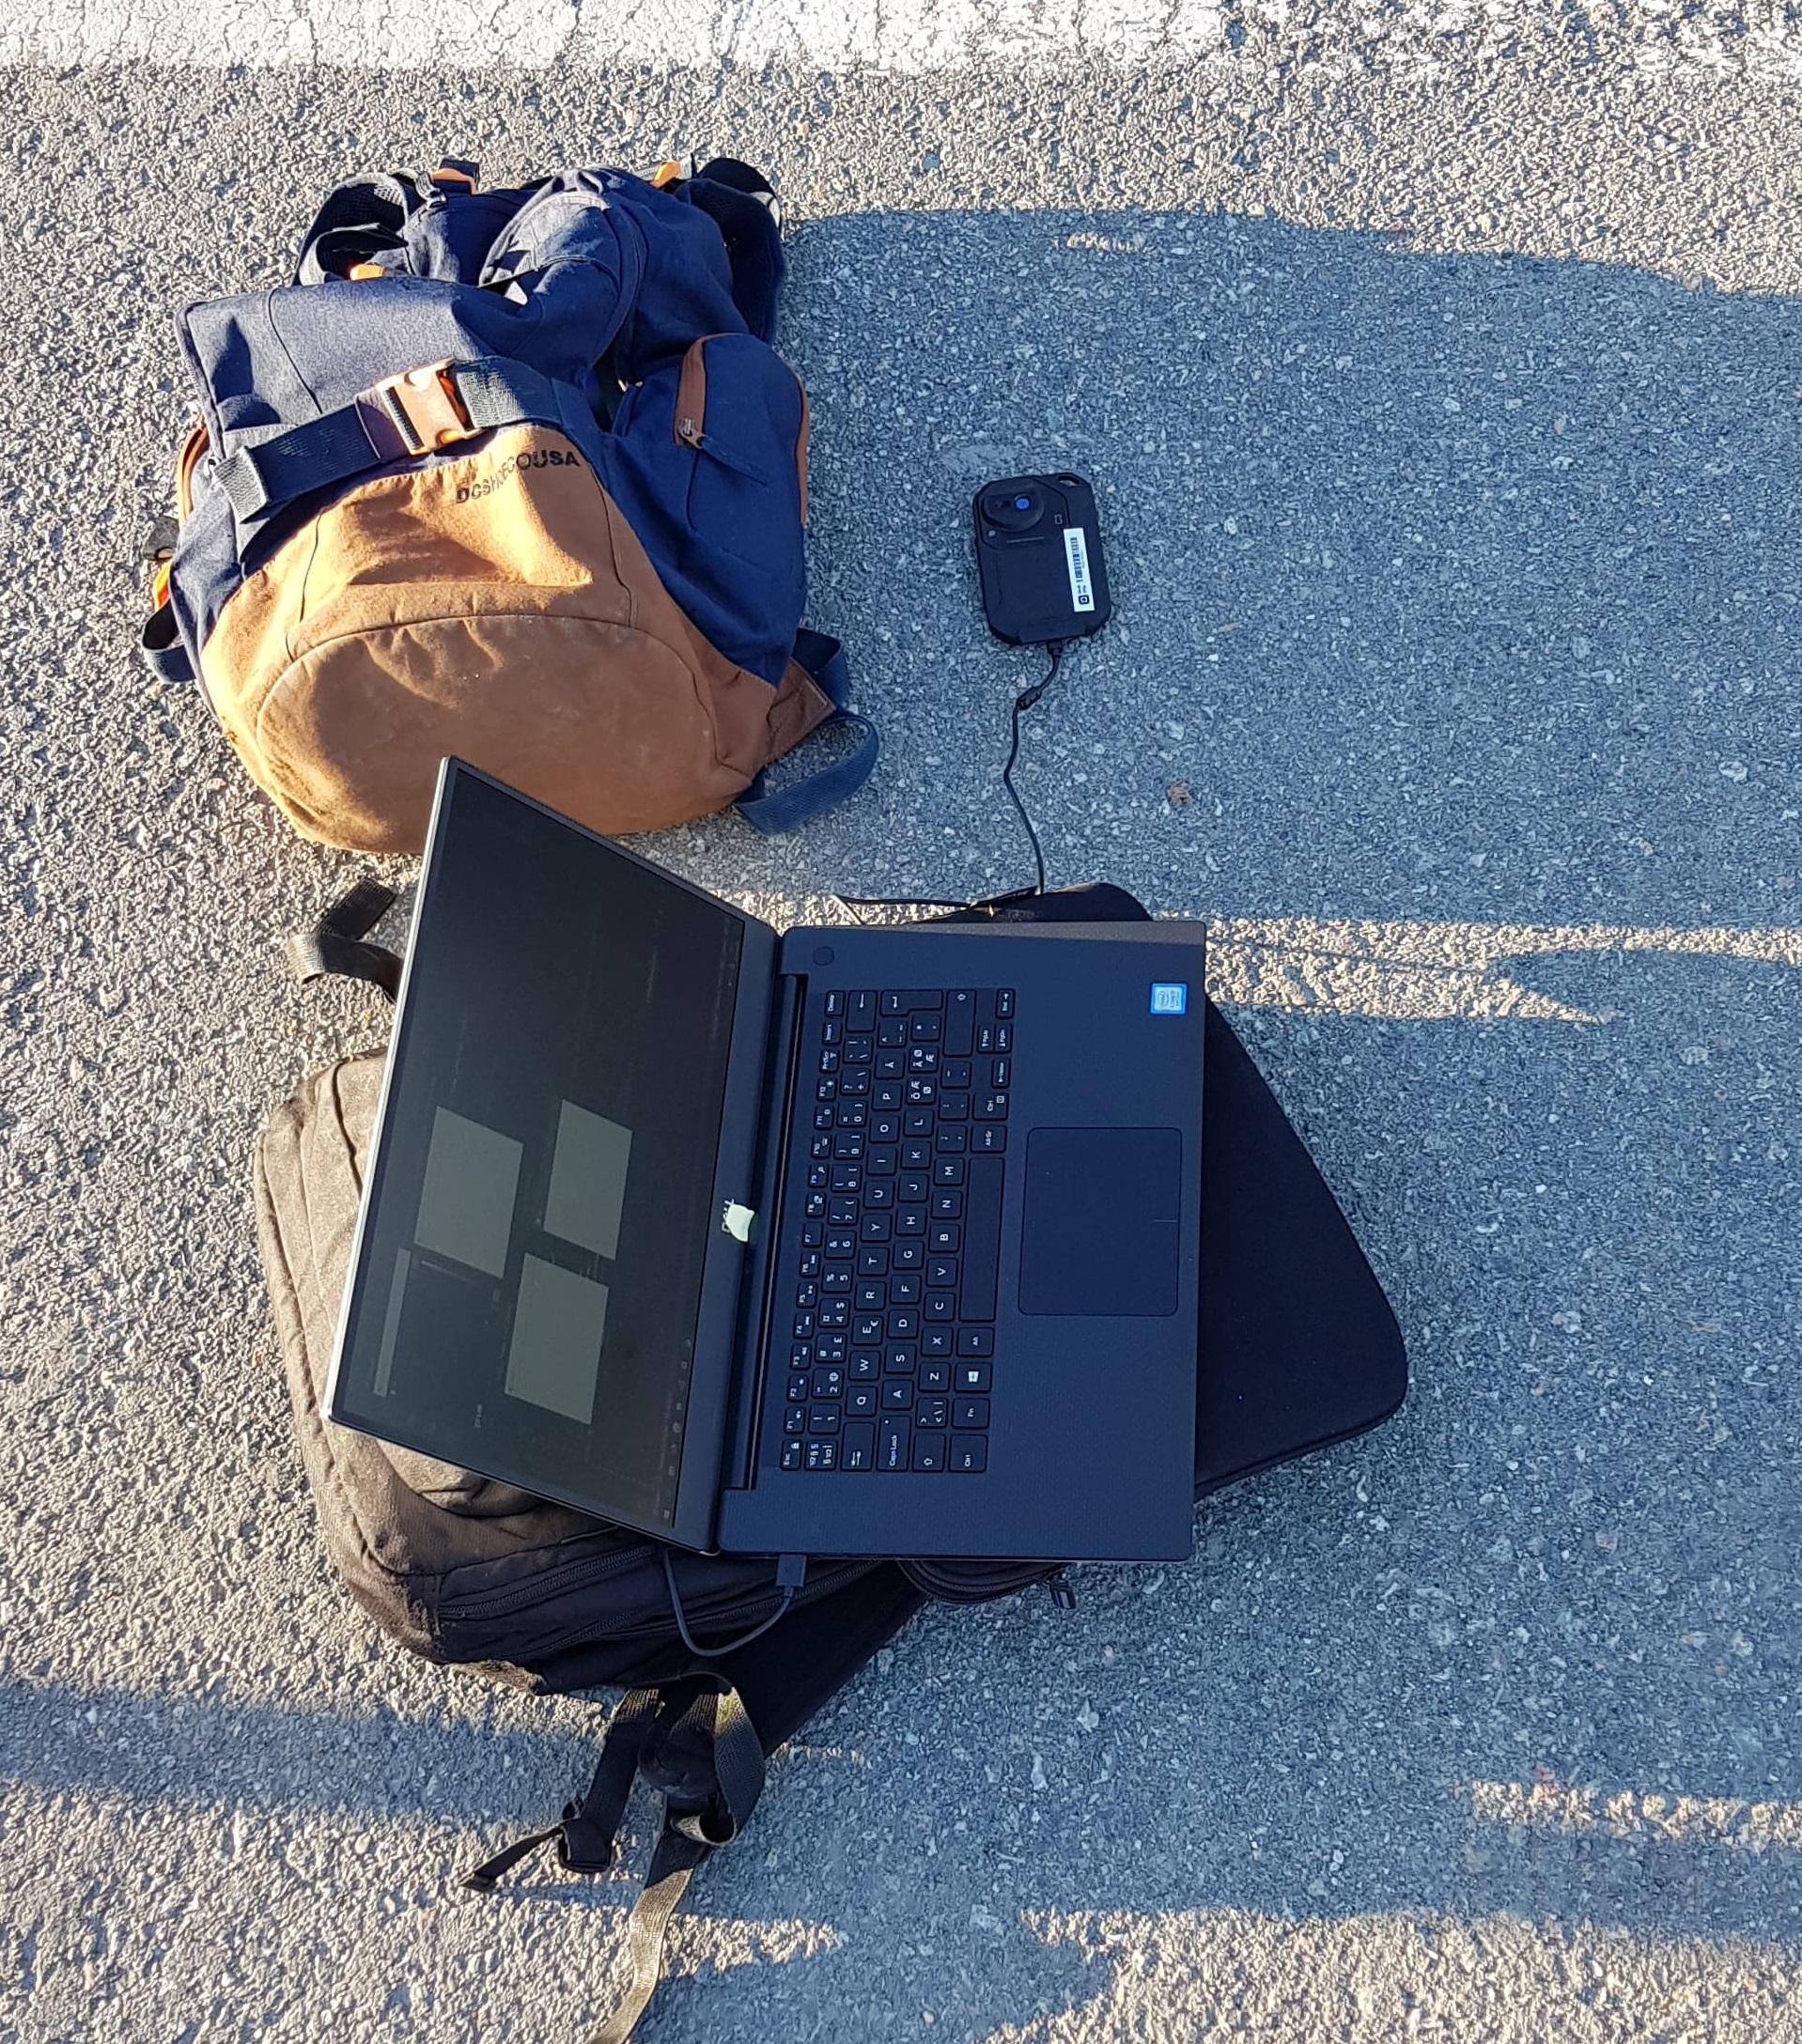
\includegraphics[width=1\textwidth]{verifikasjon-test/Testoppsett/Testoppsett5.jpg}
        \caption{Utendørs testoppsett. Kamera var koblet til en bærbar datamaskin som kjørte programvaren.}
        \label{fig:verifikasjon:testoppsett1}
    \end{minipage}\hfill
    \begin{minipage}{0.45\textwidth}
        \centering
        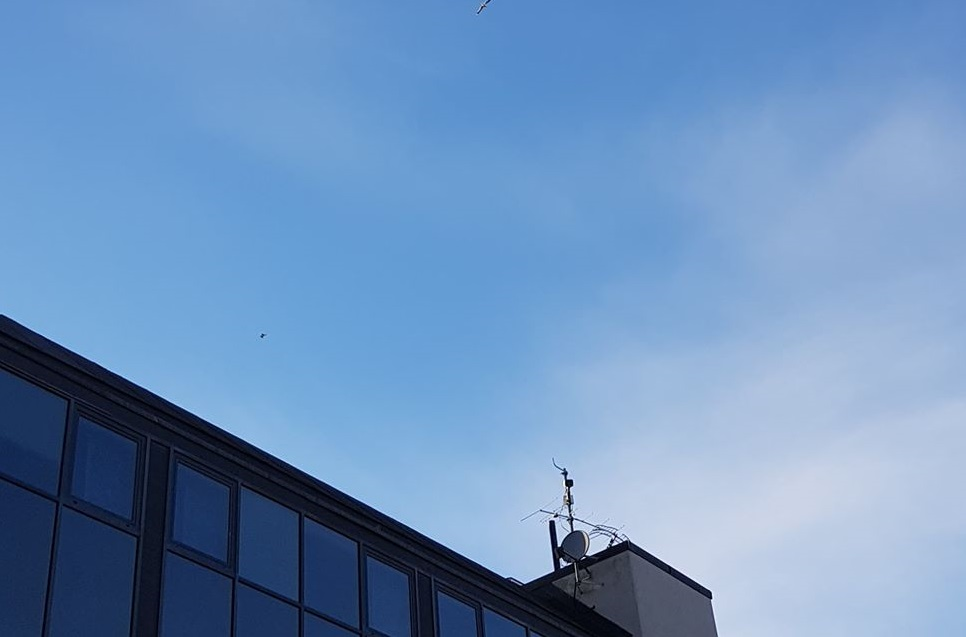
\includegraphics[width=1\textwidth]{verifikasjon-test/Testoppsett/Testoppsett6.jpg}
        \caption{Værforholdene under testing med testoppsettet i \autoref{fig:verifikasjon:testoppsett1}.}
        \label{fig:verifikasjon:værTest1}
    \end{minipage}
\end{figure}

Under test 2 var det overskyet, og kameraet var vinklet omtrent $45\degree$ fra horisontalen. Denne testen gikk i omtrent 6 timer. I tillegg til IR-kamera ble det brukt et konvensjonelt kamera for å kunne sammenlikne infrarøde og synlige bilder. Her ble ikke alle bilder analysert, men kun de bildene som ble oppdaget av programvaren til å inneholde blobs ble lagret grunnet den store mengden data. Under denne testen ble det testet hvor stort utslag overskyet vær har på resultater og tracking.

\todo{pass på at det kommer fram senere at det var få resultater fra test 2, delvis pga få fugler, delvis pga systemet hadde kort rekkevidde. pass også på å få fram at denne testen i hovedsak rettet seg mot falsk positiv fremfor negativ, og at det var kalibrering og kamerainstillinger som utgjorde 99 \% eller noe slik av alle feil}


%test1 -> oppholdsvær -> kamera pekende ca. 30-45 grader (varierte litt vinkel) -> kamera i skygge -> bærbar pc, men data ble ikke alltid overvåket live. Ble brukt gopro, men ikke hatt tid til å analsyere dette skikkelig bla bla
%Dette som ble testet lengst sammenhengende, men lite analyse av data og mye å anta at programvaren fungerte (aka lagre bilder med keypoints og se gjennom disse i ettertid, uten å sjekke gopro for å se etter fugler som burde blitt observert).
\begin{figure}[H]
    \centering
    \begin{minipage}{0.48\textwidth}
        \centering
        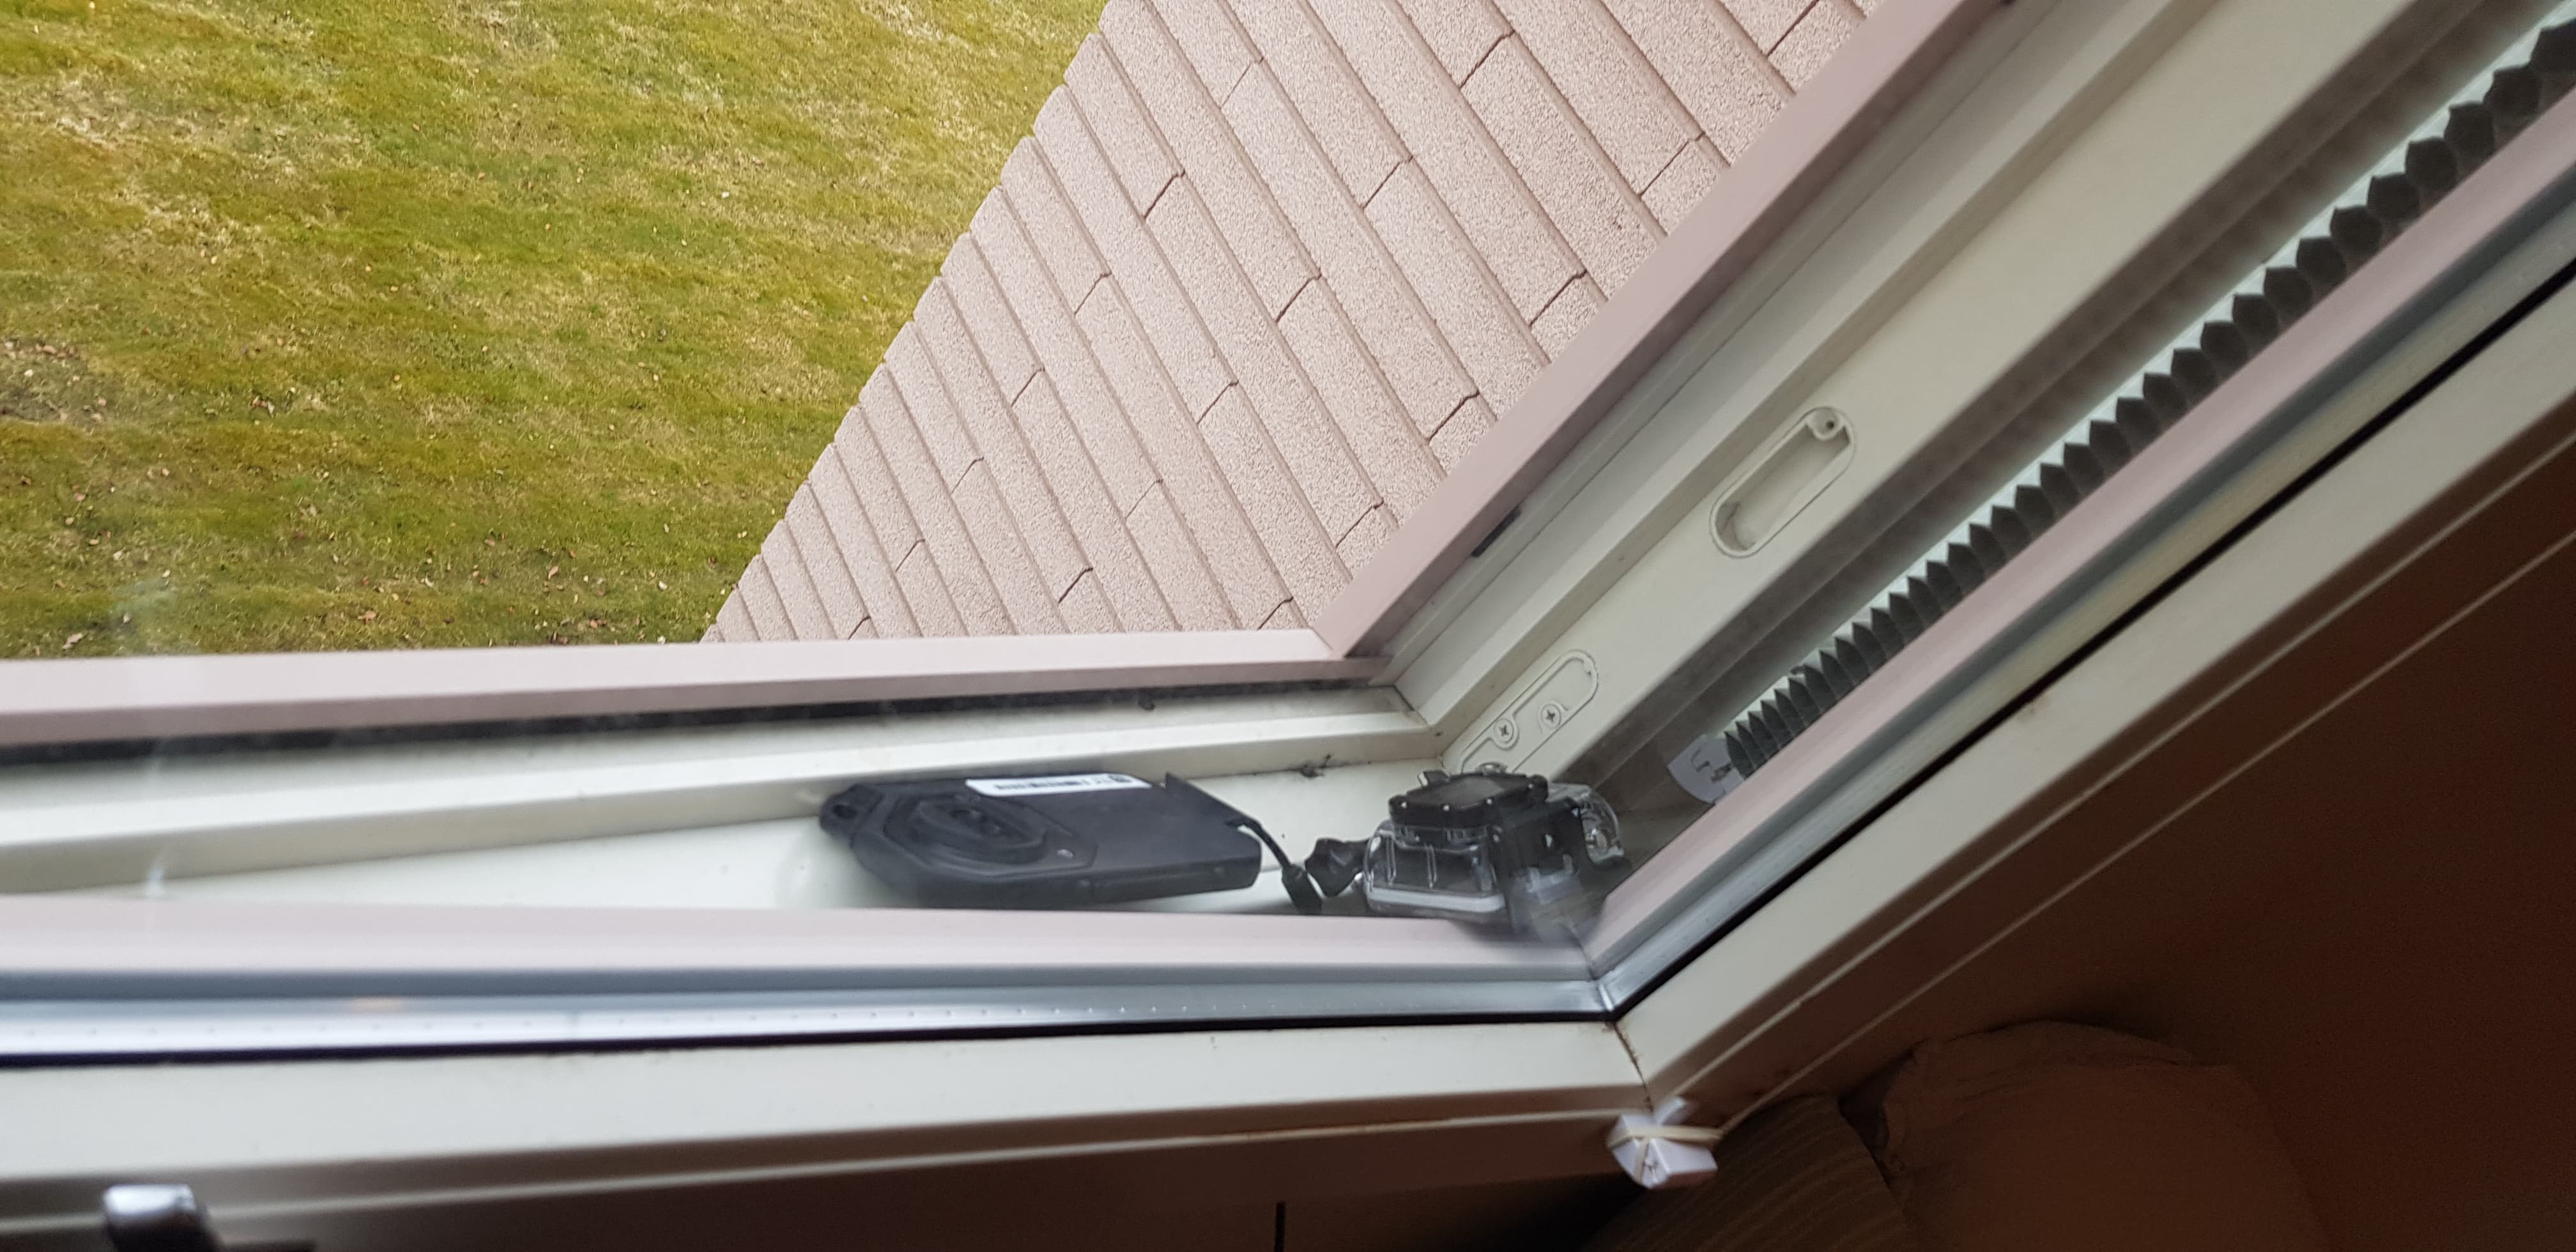
\includegraphics[width=1\textwidth]{verifikasjon-test/Testoppsett/Testoppsett1.jpg}
        \caption{Utendørs testoppsett. IR-kameraet er lagt i en vinduskarm ved siden av et kamera. Det var så koblet til en bærbar datamaskin som kjørte en modifisert programvare som lagret de bildene hvor det var detektert blobs.}
        \label{fig:verifikasjon:testoppsett2}
    \end{minipage}\hfill
    \begin{minipage}{0.48\textwidth}
        \centering
        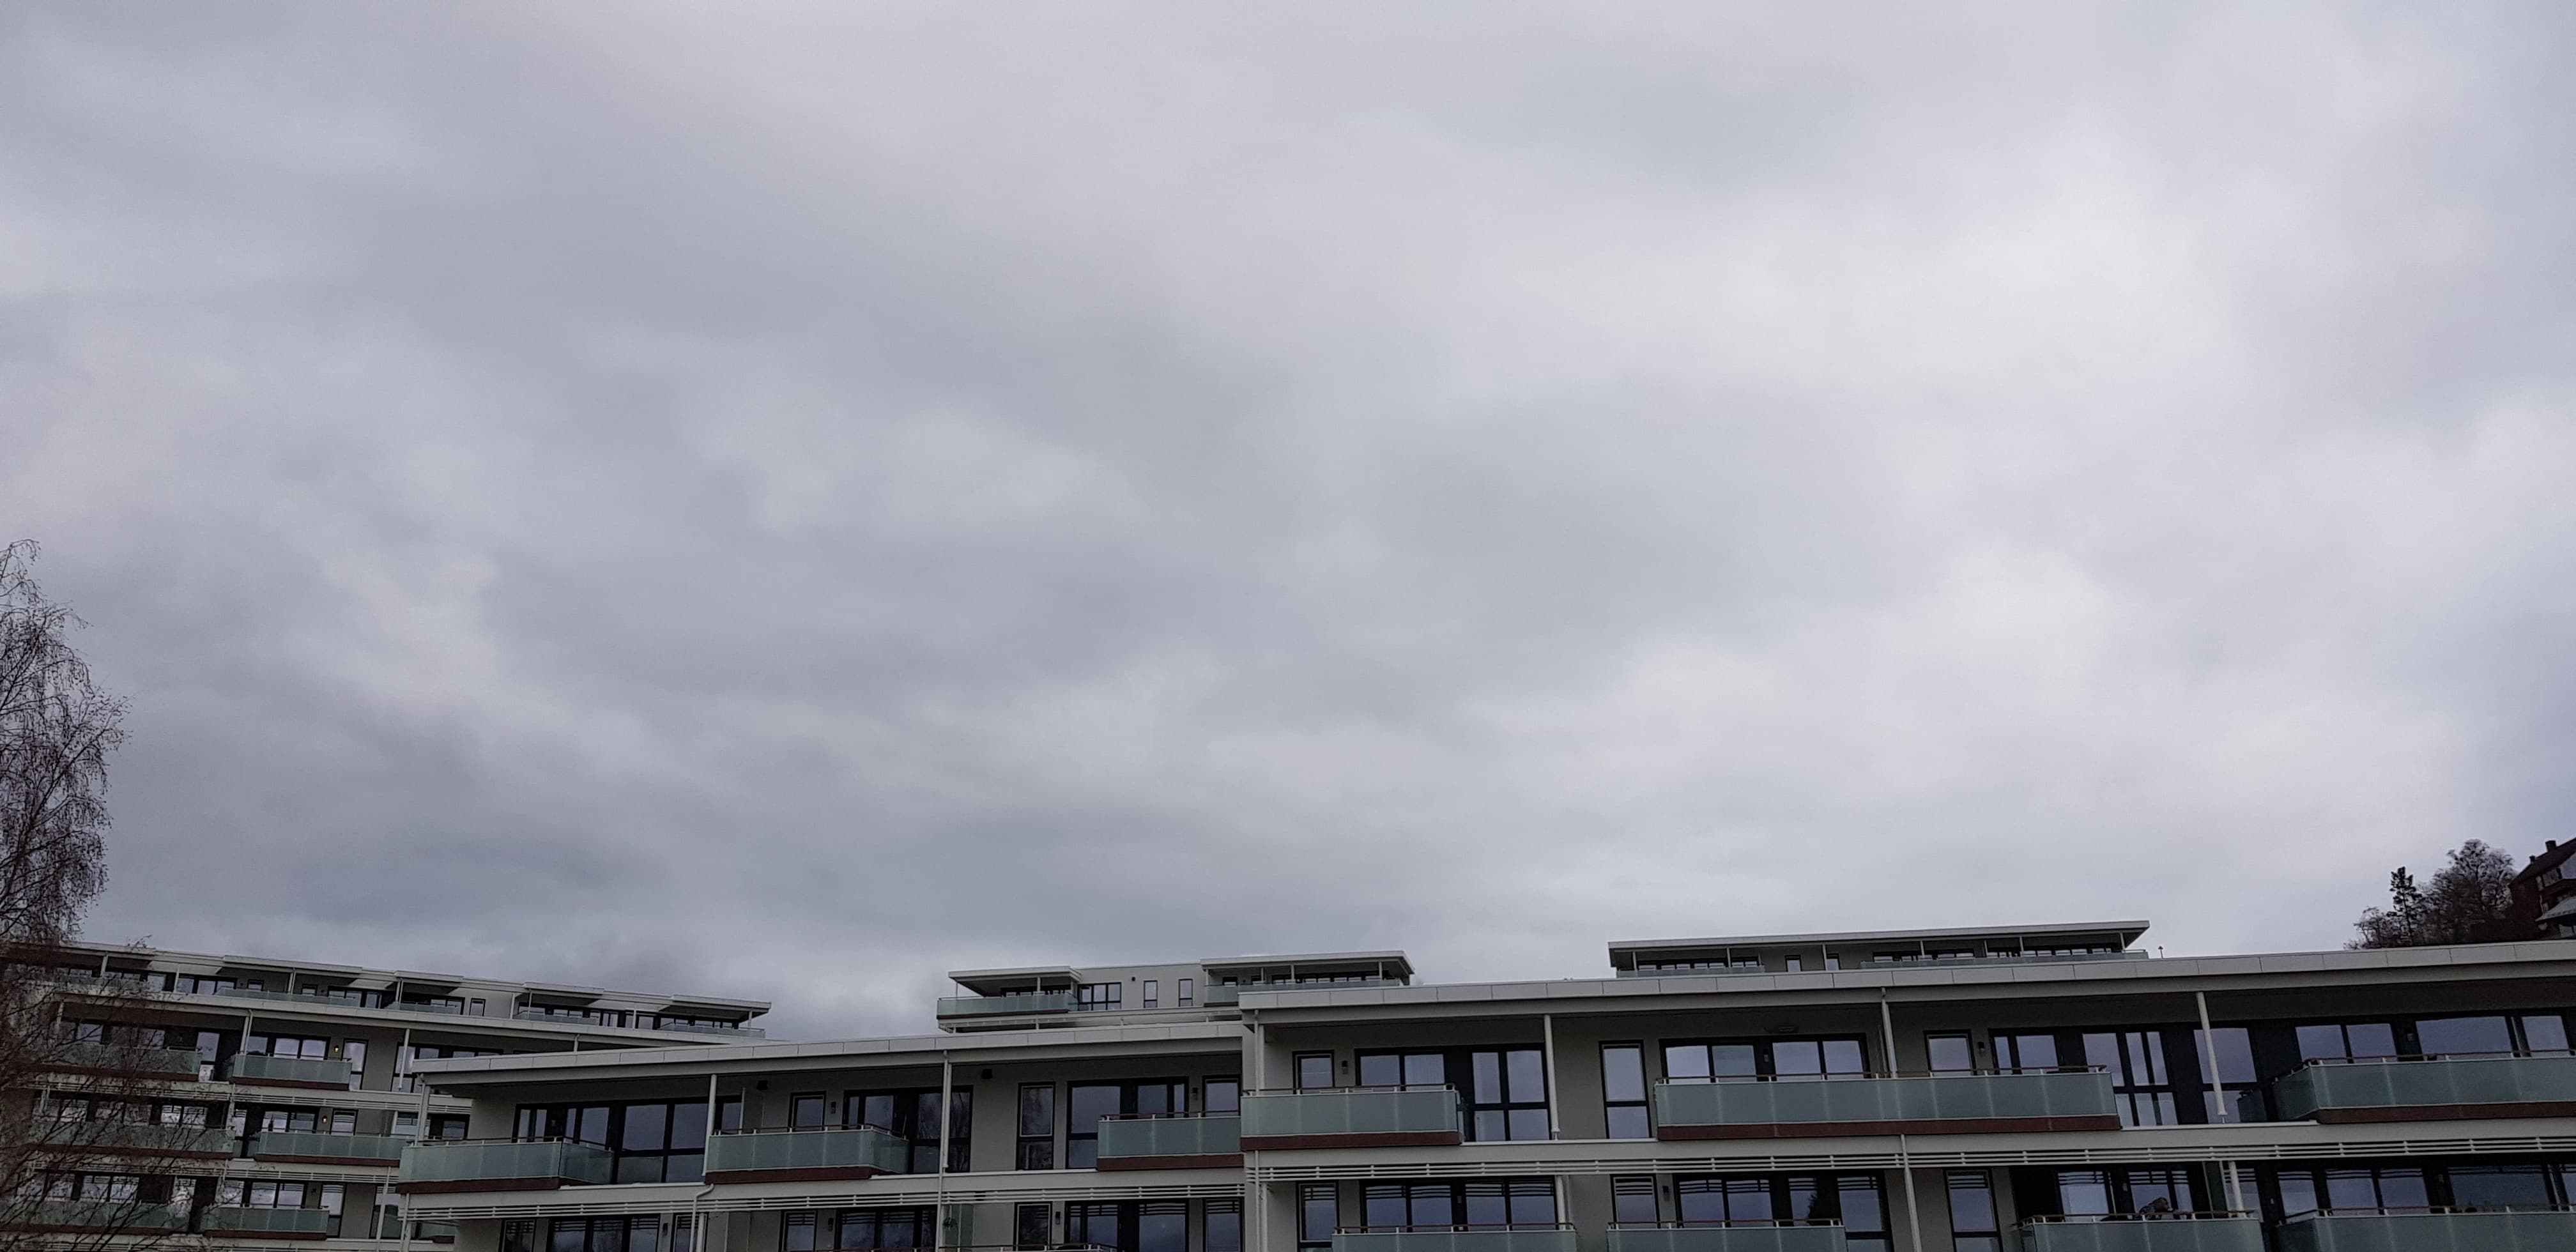
\includegraphics[width=1\textwidth]{verifikasjon-test/Testoppsett/Testoppsett3.jpg}
        \caption{Værforholdene under testing med testoppsettet i     \autoref{fig:verifikasjon:testoppsett2} var mer varierende, men det var for det meste skyet. Dette bildet er tatt med et kamera med mye bredere synsvinkel enn FLIR C3.}
        \label{fig:verifikasjon:værTest2}
    \end{minipage}
\end{figure}


\subsection{Kamera}\label{sec:verifikasjon:kamera}

Systemkrav \idref{id:kamera} er oppfylt ut fra spesifikasjonene oppgitt av FLIR. 

\subsubsection{Rekkevidde}\label{sec:verifikasjon:rekkevidde}
Kameraet har rekkevidde opp mot 30m, og kan klare å se fugler i høyder over dette. 
I \autoref{fig:verifikasjon:bilde_fugl} kan vi se et eksempel på et bilde av en fugl mot skyfri himmel. 
Det var hovedsaklig måker (ca. 50 stk.) testingen er utført på, og disse kan man tydelig se med kameraet i høyder opp til 30m. 
Dette er estimert ved å sammenligne med høyden til bygninger i området. 
Det er stor usikkerhet i høyden fuglene ble observert, men fra testingen er det ikke urealistisk at man kan observere større fugler i høyder rundt 40-50m. 
Dette betyr at systemet potensielt kan oppfylle systemkrav \idref{id:rekkevidde} gitt gode forhold.
Et av problemene ved testing av rekkevidde, er mangel på måleutstyr. 
Det er derfor ikke mulig å fastslå nøyaktig høyde for fuglene som var synlig, eller ikke synlig på bildene.
Dette gjør at systemkrav \idref{id:rekkevidde} ikke er fullstendig testet og verifisert, og fører videre til at systemkrav \idref{id:temperatur} ikke er verifisert, grunnet vanskelig verifikasjon av høyde og størrelse.

\begin{figure}[H]
    \centering
    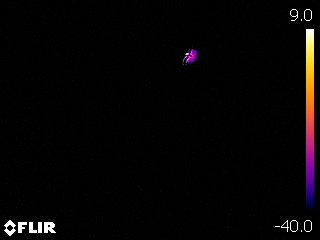
\includegraphics[width=.5\textwidth]{verifikasjon-test/Kamera/FLIR0059.jpg}
    \caption{Her kan vi se et bilde av en måke tatt med kamera. Denne fuglen var ca. 10-20m oppe i lufta. Bildet er slått sammen av et vanlig bilde og et termisk bilde med FLIR sin programvare.}
    \label{fig:verifikasjon:bilde_fugl}
\end{figure}

Rekkevidde i andre værforhold ble ikke testet like godt, men det virker som om rekkevidden er betydelig lengre når det det er skyfritt.

\subsubsection{Værforhold}\label{sec:verifikasjon:kamera:værforhold}

Kameraet ble testet mot åpen himmel og mot skyer. 
I \autoref{fig:verifikasjon:kamera_skyfri} kan vi se et eksempel på hvordan et bilde ser ut med kameraet rettet mot åpen himmel uten fugler i bildet. 
Dette gir lite støy å filtrere bort, som man tydelig kan se fra bildet. 
Dermed blir det relativt enkle bilder for filtrering, som vi for eksempel kunne se i \autoref{fig:verifikasjon:bilde_fugl}. 
Å rette kamera mot solen var mulig, men som vi vil se i \autoref{sec:verifikasjon:programvare:filtrering} fungerer trolig ikke filtreringen i programvaren godt nok til å kunne filtrere solen og fugler samtidig, selv om det ikke er gjort noen konkrete undersøkelser om dette.

\begin{figure}[H]
    \centering
    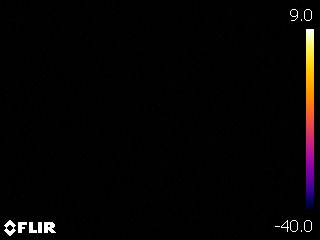
\includegraphics[width=.5\textwidth]{verifikasjon-test/Kamera/skyfri.jpg}
    \caption{Her kan vi se et bilde tatt med kameraet rettet mot en skyfri himmel. Vi kan se at det ikke reflekteres noe IR-stråling fra himmelen.}
    \label{fig:verifikasjon:kamera_skyfri}
\end{figure}

Oppgaven om å filtrere bildet blir mer krevende dersom man har skyer på himmelen. 
I \autoref{fig:verifikasjon:kamera_skyfri} ser vi at kameraet har kalibrert seg slik at skyen blir godt synlig på bildet. 

\begin{figure}[H]
    \centering
    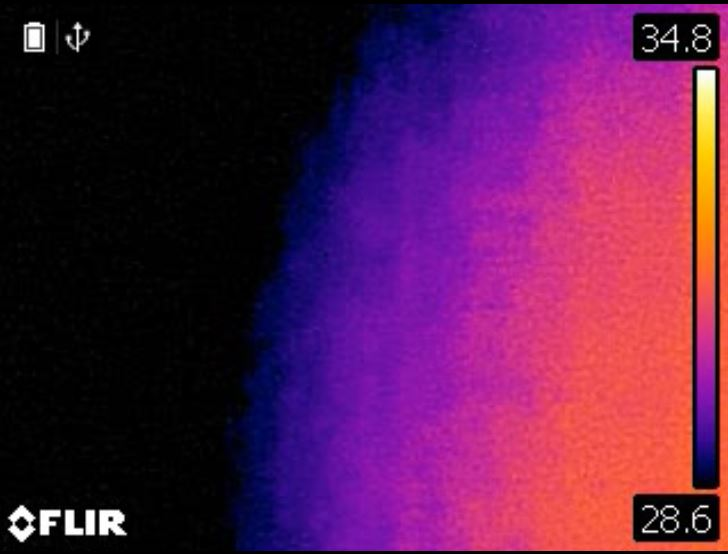
\includegraphics[width=.5\textwidth]{verifikasjon-test/Kamera/skyer3.JPG}
    \caption{Her kan vi se et bilde tatt med kameraet rettet mot kanten av en sky. Vi kan se at skyen, altså områdene med farge, gir en betydelig større utfordring når bildene skal filtreres.}
    \label{fig:verifikasjon:kamera_skyer}
\end{figure}

Vi ser at temperaturskalaen går fra $28.6-34.8 \celsius$ i \autoref{fig:verifikasjon:kamera_skyer}. 
Dersom man stiller inn kameraet til en annen skala ble dette betydelig forbedret, men det er usikkert hva dette gjør med rekkevidden til kamera, da det ikke ble mulig å teste dette i tilsvarende forhold som de i \autoref{sec:verifikasjon:rekkevidde}.



Det er også usikkert hvordan systemet fungerer i andre værforhold som snø, regn og tåke, siden det ble tatt i bruk lånt utstyr man ikke ville risikere å ødelegge, samt at værforhold som tåke og snø ikke var tilgjengelige testperioden.
Derimot har FLIR funnet ut at ved sikt på under 300 meter (synlig lys) er det neglisjerbar forskjell i synsrekkevidde mellom infrarøde instrumenter og det blotte øye \cite{tåke}.
Utfordringen ligger i refraksjon av elektromagnetiske bølger når de kommer i kontakt med regndråper eller snø \cite{refraksjon}.
Dette kan føre til en redusert sannsynlighet for at varmestråling fra fugler når fram til sensoren. I tillegg er det mulig at regn og snø kan feilaktig bli detektert av systemet som fugler.

\subsubsection{Kalibrering}\label{sec:verifikasjon:kamera:kalibrering}

Med jevne mellomrom kalibrerer kameraet seg. 
Kameraet er et kommersielt produkt, og den forhåndsinstallerte programvaren vil justere kameraet for å gi større kontrast mellom de varme områdene i et bilde. 
Dette skjer oftere dersom varme objekter raskt forsvinner ut av bildet, eller dersom det er mulig å finne store kontraster som for eksempel når det er skyer. 
Dette er ugunstig ettersom at vi ikke ønsker at kameraet skal fremkalle varmesignaturer på denne måten. 
Når kameraet kalibreres oppstår det mønstre på skjermen, som vist i \autoref{fig:verifikasjon:kalibrering}, og dette er utvilsomt noe av det som ga store feil i form av falske positiver.
Dette kunne resultere i alt fra null til flere hundre feil (falsk positiv) i timen, avhengig av værforhold og innstillinger på kameraet. 
Få til ingen feil oppsto ved skyfri himmel og godt vær, flest feil oppsto når det var skyer eller hyppige endringer i værforhold.


En test som ble utført var å peke kameraet mot en fugl, slik at man lot kameraet kalibrere seg. 
Bildene ville ofte gi tydelige kontraster mellom fugler og bakgrunn uavhengig om det var skyer eller ikke siden fuglene var mye varmere enn bakrunnen. 
Utfordringer oppsto når fulgen forsvant ut av synsfeltet til kamera, og kameraet ville forsøke å kalibrere seg mot det nye motivet. 
Dersom det var skyer ville dette ofte gi output som i \autoref{fig:verifikasjon:kalibrering} etterfulgt av støyfulle bilder som i \autoref{fig:verifikasjon:kamera_skyer} som vi undersøkte i \autoref{sec:verifikasjon:kamera:værforhold}. 
Dette var et mer ubetydelig problem ved skyfri himmel, ettersom at den nye outputen ville bli som i \autoref{fig:verifikasjon:kamera_skyfri}.
\todo{helt ubrukelig referering til figurer}

\begin{figure}[H]
    \centering
    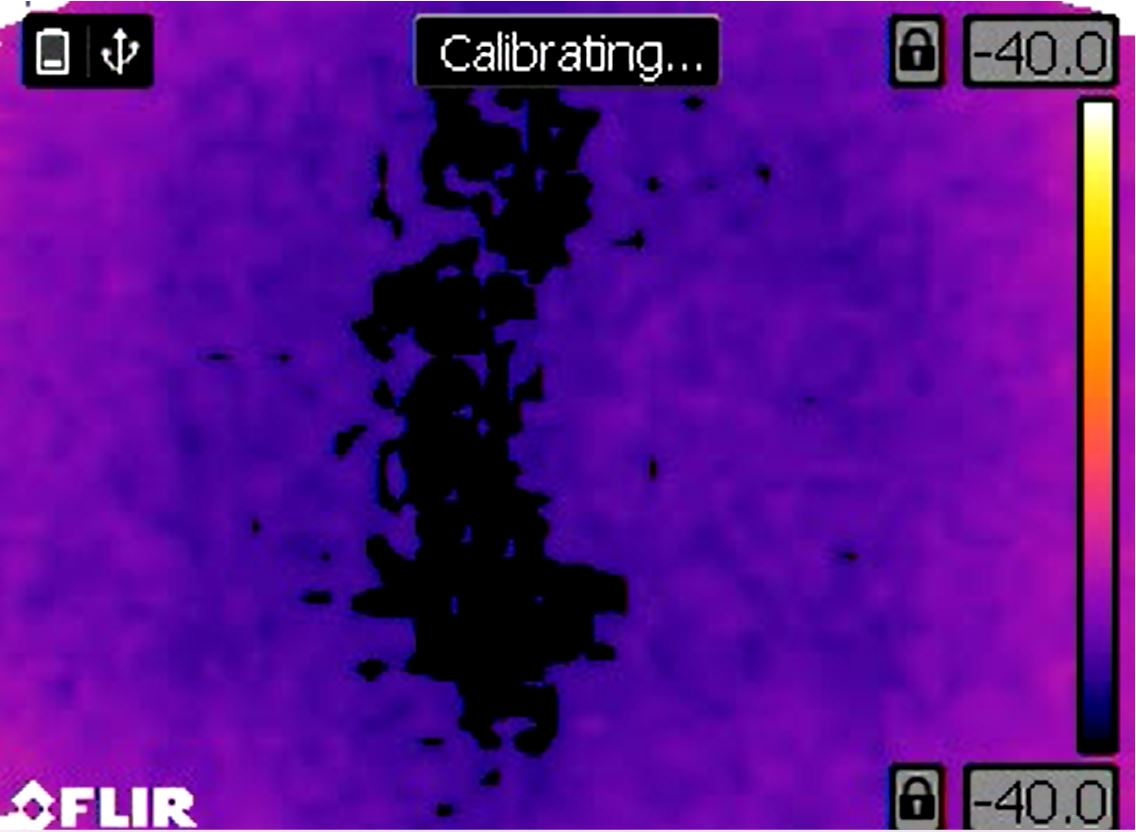
\includegraphics[width=.5\textwidth]{verifikasjon-test/Kamera/kalibrering.jpg}
    \caption{Et eksempel på hva som skjer når kamera kalibreres. Bildet inneholder mye støy.}
    \label{fig:verifikasjon:kalibrering}
\end{figure}

\todo{formater bilder bedre og skriv bedre tekst}
Når dette skjer vil mange blobs bli detektert i bildet, og det vil opprettes trackere for disse. 
Det vil føre til at programmet teller veldig mange fugler som ikke er der, i tillegg til at prosessoren ikke har nok prosessorkraft til å oppdatere alle trackerene. 

\todo{hva med overlay-ting fra flir? man burde vel nevne det også +  skrive en plass at vi bare klipte det bort}

\subsection{Prosesseringsenheten}
\todo{skriv verifikasjon om pi-en}

\textit{bare å skrive kort at opencv gikk an å laste ned + at den fungerer more or less som en vanlig data. Selv om den ikke ble testet grundig pga korona kan man sammenligne den med i7-prosessor og 16gb ram som ble brukt under testing. Få fram at det fungerte veldig bra på pc, med unntak av tracking ved feks kalibreringsfeil hvor 10 blobs kunne oppstå i samme bilde som ga lang prosesseringstid per frame. Det hadde dermed ikke vært vits å ha bedre prosesseringsenhet siden det ikke fungerte optimalt på en laptop heller -> optimalisering av kode / bedre kamera. Blob detection fungerte utmerket på pi-en og analyserte fint godt over 30 frames per sekund dersom det var realistisk mengde blobs (nærmere 10 enn 100). Går an å lage og kjøre en liten testkode for å teste fps for prosessering av ir-bilder. greit med tall.}



\subsection{Programvare}\label{sec:verifikasjon:programvare}

\subsubsection{Filtrering}\label{sec:verifikasjon:programvare:filtrering}
For skyfri himmel gir filtreringen forventet resultat. 
Vi kan for eksempel se på \autoref{fig:verifikasjon:filtrering:org} som et eksempel. 
Bildet viser 3 måker innenfor synsfeltet, alle i lav høyde (ikke målt, men et raskt estimat er rundt 15-20m).

\begin{figure}[H]
    \centering
    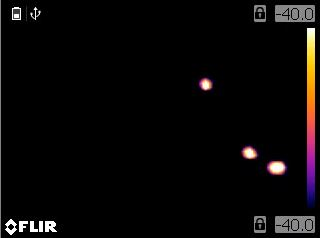
\includegraphics[width=.5\textwidth]{verifikasjon-test/Tracking_ex/org1.JPG}
    \caption{Bilde av 3 måker mot skyfri himmel.}
    \label{fig:verifikasjon:filtrering:org}
\end{figure}

Vi kan så bruke filtreringsfunksjonen på dette bildet, og får et resultat som vist i \autoref{fig:verifikasjon:filtrering:filt}.
Dette resultatet er godt egnet for \textit{blob}-deteksjon med klare \textit{blobs} på en hvit bakgrunn. I dette eksempelet hadde de tre fuglene omtrent lik varmesignatur. I ett tilfelle under testingen hadde en fugl lavere varmesignatur som følge av at den fløy høyere oppe enn to andre fugler. Denne kommer vi tilbake til i \autoref{fig:verifikasjon:long} i \autoref{sec:verifikasjon:programvare:blob-detection_og_tracking}. Fordi varmesignaturen var betydelig lavere for fuglen som fløy høyere oppe enn fuglene som fløy lavere ble denne tolket som bakgrunn og filtrert bort. Likevel klarer programvaren å detektere denne etter fuglene i forgrunnen har forsvunnet, men dette kun ut fra tilfeldighetene til hvilke fugler som kom inn og ut av bildet først.

\begin{figure}[H]
    \centering
    \fbox{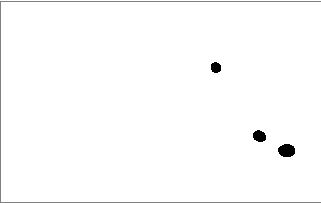
\includegraphics[width=.5\textwidth]{verifikasjon-test/Tracking_ex/filt1.JPG}}
    \caption{Filtrering av bildet i \autoref{fig:verifikasjon:filtrering:org}.}
    \label{fig:verifikasjon:filtrering:filt}
\end{figure}

\todo{legg til eksempel hvor fugl høyt oppe ble filtrert bort}

Eksempelet i \autoref{fig:verifikasjon:filtrering:filt} var tilnærmet ideelle forhold for systemet.
Dersom man for eksemel har delvis skyet vær, som vi kunne se et eksempel på i \autoref{fig:verifikasjon:kamera_skyer}, blir resultatet mindre egnet for \textit{blob}-deteksjon og \textit{tracking}.
En filtrert utgave av \autoref{fig:verifikasjon:kamera_skyer} ser vi i \autoref{fig:verifikasjon:filtering:sky}.
Resultatet i seg selv er ikke overraskende, ettersom at otzu's metode som beskevet i \autoref{sec:impl:programvare:filtrering} nettopp skal skille forgrunn fra bakgrunn.
Likevel gir dette store mengder støy og falske positiver, slik at filtreringen ikke klarer å filtrere bort en sky.
Riktignok ville ikke dette eksempelet gitt noen falske positiver, siden denne \textit{bloben} blir for stor i forhold til parameterene som ble brukt for \textit{blob}-deteksjon under testing. 
En mindre sky, eller en sky med større kontraster og lokale maksimum og minimum, kunne derimot gitt falske positiver.


\begin{figure}[H]
    \centering
    \fbox{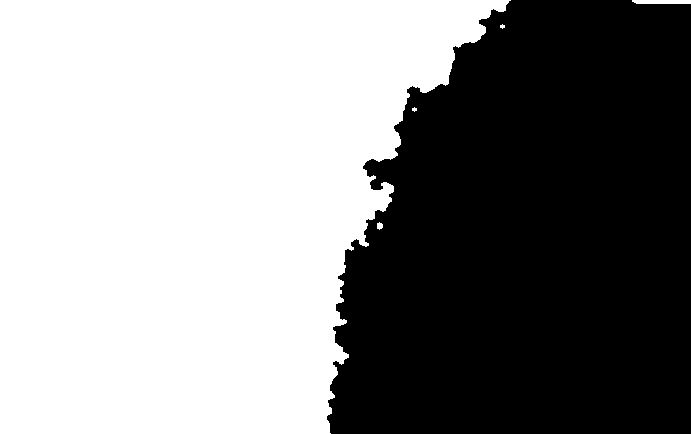
\includegraphics[width=.5\textwidth]{verifikasjon-test/Tracking_ex/filt_skyer3.jpg}}
    \caption{Skyen i \autoref{fig:verifikasjon:kamera_skyer} blir ikke filtrert bort.}
    \label{fig:verifikasjon:filtering:sky}
\end{figure}

For å skaffe en bedre forståelse av hvordan filteret oppfører seg ble det også testet med falsk data. 
Dette var hovedsaklig bilder med generert støy funnet på internett. 
\todo{kilder for disse bildene}

I \autoref{fig:verifikasjon:filter:stoy:1} ser vi et mørkt bilde, noen hvite objekter, samt en del bakgrunnstøy (enkeltpixler / små grupper pixler som er lys). 
Resultatet etter otzu's metode blir tydelige blobs på en hvit bakgrunn. 
Det ikke sikkert antallet og størrelsene til blobs er bevart, men vi ser at filtreret som en helhet utfører oppgaven med å fremheve disse.
Vi bør merke oss her at bakgrunnen i hovedsak er svært mørk i forhold til objektene.

\begin{figure}[H]
    \centering
    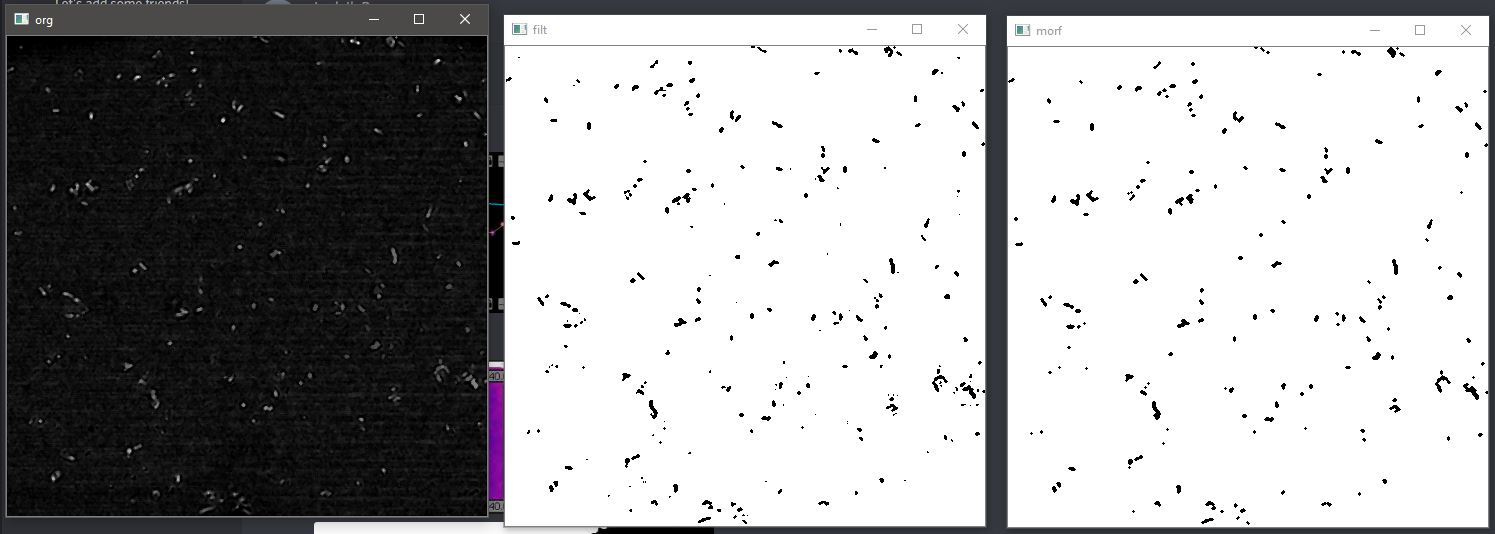
\includegraphics[width=.5\textwidth]{verifikasjon-test/Filtrering/stoy_filt1.JPG}
    \caption{Testing av filter med falsk data.}
    \label{fig:verifikasjon:filter:stoy:1}
\end{figure}

Ser vi derimot på \autoref{fig:verifikasjon:filter:stoy:2} har vi et lignende bilde, men med mer støy i forhold til eksempelet i \autoref{fig:verifikasjon:filter:stoy:1}. 
Filteret klarer ikke å filtrere dette bildet, slik at det filtrerte bildet også bare er støy uten at vi klarer å kjenne igjen noen mønster fra det originale bildet slik som i det forrige eksempelet. 
Med denne mengden støy har vi gått forbi grensen over hva som er mulig med denne implementasjonen, ettersom at filteret er implementert til å analysere hele bildet som en helhet for å bestemme en terskelverdi, fremfor å finne lokale maksimum og minimum.
\todo{ref otzu metode / implementering}

\begin{figure}[H]
    \centering
    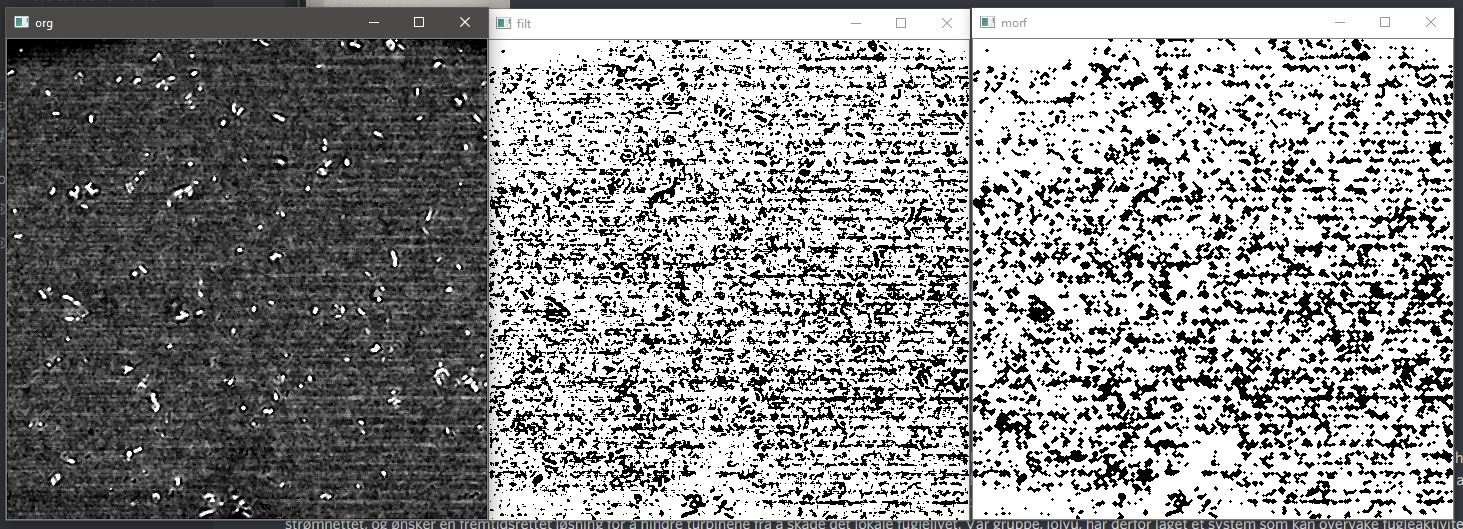
\includegraphics[width=.5\textwidth]{verifikasjon-test/Filtrering/stoy_filt8.JPG}
    \caption{Testing av filter med falsk data.}
    \label{fig:verifikasjon:filter:stoy:2}
\end{figure}

Vi kan så se på \autoref{fig:verifikasjon:filter:stoy:3}, som tydelig får fram hvordan \textit{morphology}\todo{ref implementasjon for morphology} fungerer.
Det originale bildet er allikevel støyfult, som medfører at det filtrerte bildet også har områder med støy. 
Dette gir veldig mange små \textit{blobs}. 
\textit{Morophology}-operasjonene løser dette ved å filtrere vekk små gruperinger av hvite prikker på svart bakgrunn og tilsvarende med svarte prikker på hvit bakgrunn.
Resultatet blir dermed et mye klarere bilde hvor man tydelig kan se mindre støy på de svarte å hvite områdene.
Merk at operasjonen vist i dette eksempelet er modifisert for testingen slik at den utfører sterkere og dermed mer synlig filtrering.

\begin{figure}[H]
    \centering
    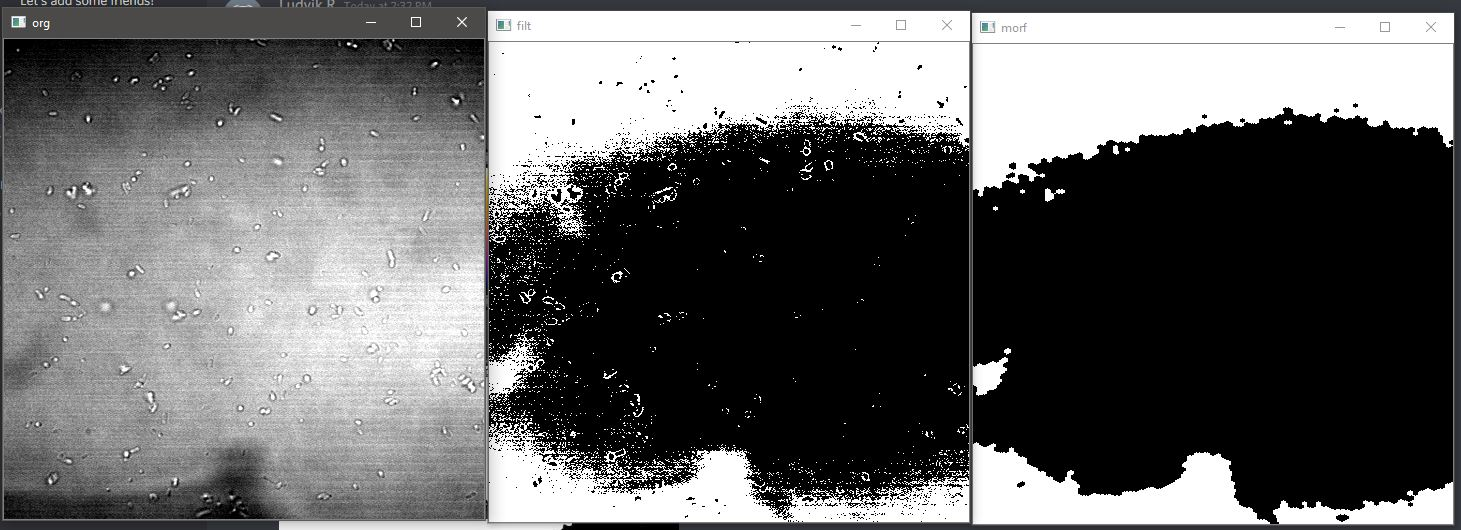
\includegraphics[width=.5\textwidth]{verifikasjon-test/Filtrering/stoy_filt4.JPG}
    \caption{falsk data testing av filter.}
    \label{fig:verifikasjon:filter:stoy:3}
\end{figure}


\todo{fiks figurene så de ser penere ut}

\subsubsection{Blob-deteksjon og tracking}\label{sec:verifikasjon:programvare:blob-detection_og_tracking}

\todo{eksempel med edge}

\todo{noter utfordring med fugler som flyr over hverandre}
Resultatene i dette kapittelet kommer fra test 1 beskrevet i \autoref{sec:verifikasjon:oppsett}.
I en testvideo med 20 fugler og skyfri himmel, klarte systemet å detektere 18 av de 20 fuglene. 
Det vil si at \textit{blob}-deteksjon oppdaget 90\% av alle fuglene i videostrømmen. 
Av disse 18 fuglene som ble detektert klarte \textit{trackinga} å følge 15 av fuglene helt til de forsvant ut av skjermen. 
På tre av fuglene mistet \textit{trackeren} fuglen en gang, og startet en ny \textit{tracker}. 
De tre fuglene ble altså telt to ganger hver. 
\textit{Trackingen} fungerte i $83\%$ av de tilfellene den fikk kjøre.
Resultater vises i \autoref{tab:verifikasjon:blobtrack:resultater}

\begin{table}[!htbp]
\centering
\caption{Delresultater og totalresultater fra testing av \textit{blob}-deteksjon og \textit{tracking}.}
\label{tab:verifikasjon:blobtrack:resultater}
\begin{tabular}{|l|l|l|l|l|}
\hline
\textbf{Delsystem} &
  \textbf{\begin{tabular}[c]{@{}l@{}}Fugler inn \\ i delsystem\end{tabular}} &
  \textbf{\begin{tabular}[c]{@{}l@{}}Fugler oppdaget \\ av delsystem\end{tabular}} &
  \textbf{\begin{tabular}[c]{@{}l@{}}Prosentandel \\ i delsystem\end{tabular}} &
  \textbf{\begin{tabular}[c]{@{}l@{}}Prosentandel \\ totalt\end{tabular}} \\ \hline
\textit{Blob}-deteksjon & $20$ & $18$ & $90\%$ & $90\%$ \\ \hline
\textit{Tracking}       & $18$ & $15$ & $83\%$ & $75\%$ \\ \hline
Hele systemet           & $20$ & $15$ & $75\%$ & $75\%$ \\ \hline
\end{tabular}
\end{table}

Systemet telte totalt 15 av 20 fugler, altså $75\%$ av fuglene, uten feil. Dette ligger innenfor systemkrav \idref{id:treffrate}.
I to tilfeller telte den ikke fuglen som fløy i bildet og i tre tilfeller telte den fuglen to ganger. 
Det betyr at etter de 20 fuglene hadde flydd forbi, hadde 21 fugler blitt telt av systemet. 
Figur \ref{fig:verifikasjon:blob:1} viser systemet som korrekt identifiserer 3 blobs. 
Figur \ref{fig:verifikasjon:tracking:1} viser at systemet korrekt tracker 3 blobs.
\todo{pass på at systemkrav kun er oppfylt i godt vær}
%se kommentar for todo under
\todo{Er det egentlig noe forskjell mellom disse figurene? - Nei, se kommentaren ved plasseringen til denne}
%nei, så bruk blob detection for å forklare at blob detection er verifisert og fungerer som forventet, med edge-tiilfellet hvor en blob er ved kanten / halvveis utenfor. Også la den fantastiske figuren til jostein fikse resten (altså tracking)

Trackingen har ikke blitt testet godt nok når det har vært overskyet, men dersom filtreringen klarer å fjerne bakgrunnen helt, vil trackingen fungere som på skyfri himmel. 
Om det derimot vil bli med forstyrrelser fra skyene i den filtrerte videostrømmen, vil trackingen få større problemer med å følge fuglene.


\begin{figure}[H]
    \centering
    \fbox{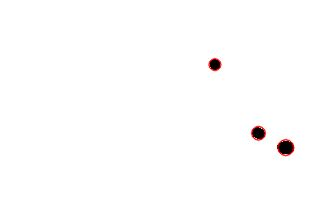
\includegraphics[width=.5\textwidth]{verifikasjon-test/Tracking_ex/blobs1.JPG}}
    \caption{Programvaren identifiserer 3 blobs og markerer disse mer rød ring.}
    \label{fig:verifikasjon:blob:1}
\end{figure}
\begin{figure}[H]
    \centering
    \fbox{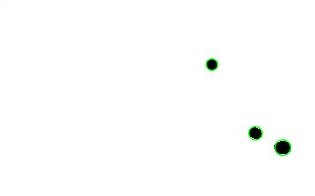
\includegraphics[width=.5\textwidth]{verifikasjon-test/Tracking_ex/track1.JPG}}
    \caption{Tracking.}
    \label{fig:verifikasjon:tracking:1}
\end{figure}

Et lengre utdrag av testvideoen er vist i \autoref{fig:verifikasjon:long}, med IR-bildene til venstre og den filtrerte dataen til høyre. 
En fugl (rød) som allerede var oppdaget før bilde nummer 1 i serien trackes feilfritt fram til bilde 10. 
Fuglen er synlig i bilde 11 også, men er for nærme kanten av bildet til å trackes, før den forsvinner ut av kameraets synsfelt i bilde 12.
En annen fugl (blå) blir synlig i bilde 7 og trackes til bilde 8. Mellom bilde 8 og 9 brytes trackingen, og fuglen tolkes i bilde 9 som en ny fugl. Den trackes så fram til bilde 12, hvor bildeserien slutter. Det at fuglen oppdages på nytt vises i den filtrerte dataen som en blå kant rundt objektet, der objekter som trackes fra forrige bilde har grønn kant.
En fugl som enten er mindre eller lengre unna enn de to andre (gul) er også synlig i kameraet fra bilde 8 til 12, men den har blitt filtrert bort, og oppdages dermed aldri. 

\begin{figure}[H]
    \centering
    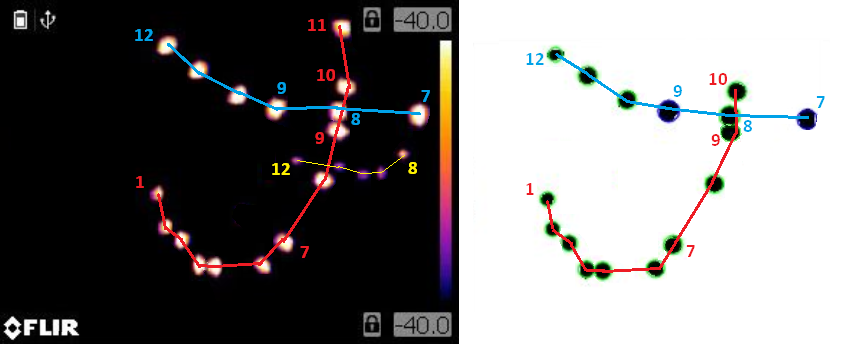
\includegraphics[width=.8\textwidth]{verifikasjon-test/Tracking_ex/langt_eksempel.png}
    \caption{Et lengre eksempel på tracking av fugler fra IR-bilder.}
    \label{fig:verifikasjon:long}
\end{figure}


\subsection{Værstasjon}\label{sec:verifikasjon:telemetri}
Kommunikasjon mellom Pi-en og de ulike sensorene er oppnådd, og sensorene sender ut fornuftig data. Kommunikasjonen med databasen er også testet og fungerer.
Da det ikke har vært mulig å 3d-printe boksen til systemet etter at NTNU ble stengt, har værstasjonen kun blitt testet inne. 

Temperatursensoren er verifisert ved å sammenligne med en kommersiell temperaturmåler, og lufttrykket ser realistisk ut sammenlignet med værvarsel fra \url{yr.no} på det aktuelle tidspunktet fra teststedet.
Grunnet mangel på en kommersiell luftfuktighetsensor, har denne dataen ikke blitt verifisert mot et troverdig resultat.
Det er alikvel naturlig å anta at sensoren fungerer som spesifisert i databladet\cite{bme280}, da sensoren sender ut realistisk data og den registrerte luftfuktigheten øker når man blåser på sensoren.
Da luftfuktigheten registreres av samme komponent som temperaturen og lufttrykket som er verifisert, underbygger dette ytterligere at luftfuktighetssensoren gir riktig data.

Nedbørsmåler er verifisert ved å helle vann over den, mens vindretnings- og vindhastighetsmåleren er testet ved å manuelt snu på dem.

Dette oppfyller systemkrav \idref{id:telemetri}.

\todo{savner noen konkrete tall her. Har man et eksempel for måling vs. yr feks? tilsvarende for temperatur}

\subsection{Nettside og database}\label{sec:verifikasjon:nettside}

Fordi systemet ikke er testet i sin helhet over lengre tid ble databasen fylt med testdata. 
Denne dataen er generert slik at en kan se forskjell på dataen. 
Programmet som genererer testdataen ligger også i jolyu sin GitHub \cite{GitHub}, under \texttt{nettside/data}. 
Nettsiden leser denne dataen og produserer grafer som visualiserer dataen på en fornuftig måte, og oppfyller derfor systemkrav \idref{id:nettside}. 

Overføring av data fra prosessorenhet er også testet ved å skrive værdata og telemetri til databasen. 
Dette fungerer også slik som det skal, og dermed oppfyller systemkrav \idref{id:eksternoverføring}.


\subsection{Systemet som en helhet}\label{sec:verifikasjon:helhet}
Systemkrav \idref{id:mål} og \idref{id:opensource} er oppnådd, siden systemet utfører oppgavene sine. 
Igjen så er dette gjort med testdata, siden systemet ikke er testet met ekte data som helhet.



\subsection{Komplikasjoner ved testing}\label{sec:verifikasjon:kowona}
%uwu pls fowgive us s-senpaii baka *w* pwetty pwease cowona got us bad}
%baka *w* pwetty pwease cowona got us bad ~rawrrrr~ :3 

Grunnet koronapandemien våren 2020 var det enkelte ting som var planlagt å teste, som vanligvis ville vært mulig å teste, men som ikke lot seg gjennomføre. 
Mangel på 3D-printer førte til at produktets ytre struktur ikke ble konstruert, slik at det ikke lot seg teste i hvilken grad denne er værbestandig, altså systemkrav \idref{id:IPrating}. 
Strukturens design er laget for å være mest mulig vanntett og værbestandig, men uten testing er dette vanskelig å fastslå.

Det var heller ikke mulighet for å sette alle systemets strukturelle deler sammen, slik som å feste boks og sensorer til stativ og sette det utendørs til testing.
Det største problemet var at testing av et komplett system ble umulig, da utstyr ble spredt mellom gruppemedlemmer for å kunne fortsette arbeid hver for seg rundt om i Norge. 
Systemkrav \idref{id:størrelse} er gjennomført i den grad at boksen er designet, men ikke 3D-printet. 
